\documentclass[12pt,oneside,openany]{report}
\usepackage[a4paper,width=150mm,top=25mm,bottom=25mm]{geometry}
\usepackage{fontspec}
\setmainfont{Times New Roman}
\usepackage{polyglossia}
\setdefaultlanguage{english}
\usepackage{csquotes}
\usepackage{amsmath}
\usepackage{graphicx}
\usepackage{caption}
\usepackage{array}
\usepackage{booktabs}
\usepackage{longtable}
\usepackage{hyperref}
\hypersetup{colorlinks=true,linkcolor=black,urlcolor=black,citecolor=black}
\graphicspath{{images/}}
\setlength{\parindent}{0em}
\setlength{\parskip}{0.6em}
\usepackage[backend=bibtex,style=ieee,sorting=ynt]{biblatex}
\addbibresource{bibliography/references.bib}

\begin{document}

\begin{titlepage}
\centering
{\Large Civic.ai: A Bilingual Retrieval-Augmented Generation System for Bangladeshi Government-Service Question Answering\\[1cm]}
{\large Merged Draft from Phase 1 and Phase 2\\[0.5cm]}
{\large Prepared for thesis review and future integration into the official template\\[2cm]}
{\large Current implementation domain: Birth and Death Registration\\[0.5cm]}
{\large Date: June 2026}
\end{titlepage}

\phantomsection
\addcontentsline{toc}{chapter}{Abstract}
\section*{Abstract}

Accessing government-service information in Bangladesh is often difficult because service procedures, fees, legal rules, correction instructions and frequently asked questions are scattered across different portals, documents and formats. Citizens may ask questions in Bangla, English or code-mixed language, while source documents are often noisy, Bangla-heavy and affected by formatting, OCR or encoding issues. A general chatbot is not sufficient for this setting because fluent answers without reliable evidence can create misinformation in public-service guidance.

This thesis proposes Civic.ai, a bilingual Retrieval-Augmented Generation (RAG) based question-answering system for Bangladeshi government services. The current phase focuses on the birth registration domain as the first testable implementation. The system uses a modular pipeline consisting of data collection, manual and semi-manual cleaning, document-type-aware chunking, metadata preservation, dense embedding, sparse retrieval, rank fusion, reranking, safe answer path checking and local LLM-based answer generation. To improve retrieval while preserving factual grounding, each chunk is represented using two separate text fields: \texttt{retrieval\_text} for search and \texttt{answer\_evidence} for generation.

The Phase 2 implementation evaluates multiple retrieval alternatives, including BM25-only retrieval, dense-only retrieval and hybrid RRF retrieval. A curated Bangla evaluation set with paraphrased citizen-style questions is used to measure retrieval behavior using Hit@k/Recall@k, Mean Reciprocal Rank (MRR), normalized Discounted Cumulative Gain (nDCG) and context precision. Preliminary results show that dense-only retrieval currently performs strongest for the single-domain birth registration dataset, while the full CivicRAG design remains important for explainability, source grounding and future multi-domain expansion. The system is implemented with local LLM backends such as llama3.2, llama3 and qwen2.5:7b so that the prototype can be tested without depending on external API keys.

The work contributes a practical and academically defensible design process for a Bangla-priority civic-service RAG system. It emphasizes factual correctness, retrieval quality, explainability, multilingual support and evaluation-driven design rather than general-purpose chatbot fluency.

\vspace{1cm}
\textbf{Keywords:} Retrieval-Augmented Generation, Civic AI, Bangla NLP, Government Services, Dense Retrieval, BM25, Reciprocal Rank Fusion, Local LLM
\pagebreak


\tableofcontents
\listoffigures
\listoftables
\clearpage

\chapter{Introduction}
\section{Introduction}
This chapter presents the background, motivation, problem statement, objectives, scope, and methodological direction of the thesis. The project, Civic.ai, is designed as a bilingual and evidence-grounded government-service question-answering system for Bangladesh. The work began with a broad idea of an AI-powered civic assistant, but the current thesis direction is more specific: building and evaluating a Retrieval-Augmented Generation (RAG) based chatbot that retrieves trusted government-service evidence before producing an answer.

The main focus of the current phase is the birth and death registration domain. This narrow scope is intentional. Government-service information is sensitive because inaccurate guidance can waste time, money, and trust. Therefore, before expanding to future domains such as passport, BRTA, birth certificate, death certificate, or other public services, the thesis first studies whether a carefully designed RAG system can provide grounded and explainable answers for one domain.

\section{Background}
Digital government services are now an important part of public administration. Bangladesh has introduced many online portals and digital services to make public service delivery more accessible. However, citizens still face practical difficulties while using these systems. Information is often scattered across multiple websites, service portals, notices, PDF files, FAQ pages, and legal documents. Many documents contain Bangla, English, mixed-language terms, tables, scanned pages, or formatting noise. As a result, even when information is technically available online, it is not always easy for ordinary citizens to find, understand, and apply.

Recent progress in natural language processing has made conversational systems more capable. The Transformer architecture introduced self-attention as a scalable method for language modeling \cite{vaswani2017attention}. Large language models such as LLaMA show that open-weight models can be used for local language generation tasks \cite{touvron2023llama,dubey2024llama3}. Bangla-focused models and resources, such as BanglaBERT, show the importance of language-specific modeling for low-resource languages like Bangla \cite{bhattacharjee2021banglabert}. However, general-purpose LLMs alone are not enough for government-service question answering because they may hallucinate or produce unsupported claims.

Retrieval-Augmented Generation addresses this limitation by connecting a language model with an external knowledge source. In a RAG system, the retriever first finds relevant evidence from a document collection, and the generator then uses that evidence to produce an answer \cite{lewis2020rag}. This design is suitable for Civic.ai because factual correctness, source grounding, and explainability are more important than creative fluency.

\section{Rationale of the Study or Motivation}
The motivation for this research comes from both social need and technical opportunity. From the citizen's perspective, many government-service procedures remain difficult to understand. People often depend on unofficial intermediaries to fill forms, understand requirements, or know where to go next. This can increase cost, delay, confusion, and risk of misinformation.

From the technical perspective, RAG provides a practical way to build a trustworthy assistant without fine-tuning a large model on every government document. Instead of depending only on the model's internal memory, Civic.ai retrieves evidence from curated government-service documents. This allows the system to be updated when documents change, makes answers easier to audit, and supports source-based verification.

The academic motivation is to study how a bilingual Bangla-English RAG pipeline can be designed for noisy real-world government documents. Unlike clean tutorial datasets, government-service data includes PDFs, converted DOCX files, HTML pages, FAQs, tables, notices, legal rules, scanned documents, encoding problems, and repeated web boilerplate. Therefore, this thesis emphasizes data cleaning, document-type-aware chunking, metadata handling, retrieval evaluation, and grounded answer generation.

\section{Problem Statement}
Despite the growth of e-government services, citizens in Bangladesh still face several barriers:

\begin{itemize}
    \item \textbf{Dispersed information:} Service instructions, document requirements, fees, and correction procedures are spread across different pages and document formats.
    \item \textbf{Language and wording barriers:} Citizens may ask in Bangla, English, or code-mixed language, while source documents may use formal Bangla, English terms, or official phrases.
    \item \textbf{Document noise:} Government pages often include menus, footers, accessibility text, duplicated links, scanned content, and formatting artifacts that can damage retrieval quality.
    \item \textbf{Lack of interactive guidance:} Existing portals mostly provide static pages or FAQs, not scenario-based conversational support.
    \item \textbf{Risk of hallucination:} A general chatbot may produce fluent but unsupported answers, which is unsafe for public-service guidance.
\end{itemize}

\textbf{Research Problem:} How can a bilingual, retrieval-based AI assistant be designed and evaluated so that it gives accurate, source-grounded, and explainable answers for Bangladeshi government-service questions?

\section{Objectives}
\textbf{Overall Objective:} To design, implement, and evaluate Civic.ai, a bilingual RAG-based government-service question-answering system that prioritizes factual correctness, retrieval quality, and explainability.

\textbf{Specific Objectives:}
\begin{itemize}
    \item Build a modular RAG pipeline with clear separation between ingestion, cleaning, chunking, embedding, retrieval, reranking, generation, and evaluation.
    \item Prepare a Bangla-heavy government-service knowledge base from noisy real-world sources.
    \item Design document-type-aware chunking for FAQ, rule, fee-table, application-process, and correction-process documents.
    \item Evaluate dense retrieval, BM25 retrieval, and hybrid retrieval alternatives using retrieval metrics such as Hit@k/Recall@k, MRR, nDCG, and context precision.
    \item Compare local LLM backends such as llama3.2, llama3, and qwen2.5:7b for grounded answer generation.
    \item Produce answers with source IDs, retrieval scores, and official links so that users and evaluators can inspect the evidence.
\end{itemize}

\section{Methodology in Brief}
The thesis follows an iterative design and evaluation methodology. First, raw government-service documents are collected from official and related sources. Second, the documents are manually and semi-manually cleaned to remove noise, duplicate navigation text, encoding issues, and irrelevant fragments. Third, cleaned files are converted into typed chunks according to document structure. Fourth, each chunk is stored with metadata and two text versions: a search-optimized \texttt{retrieval\_text} and an original \texttt{answer\_evidence} field for grounding.

The retrieval pipeline uses multilingual dense embeddings through BAAI/bge-m3 \cite{chen2024bgem3}, a sparse BM25 index \cite{robertson2009bm25}, and rank fusion through Reciprocal Rank Fusion \cite{cormack2009rrf}. The answer generation layer uses local Ollama models so that the system can run without external API keys. Evaluation is performed in two parts: retrieval-side evaluation using a curated Bangla question set, and generation-side evaluation through faithfulness, relevance, correctness, stability, and manual qualitative review.

\section{Scope and Challenges}
The current implementation scope is limited to the birth and death registration domain. This includes application procedures, correction guidance, fees, FAQ entries, legal rules, and general service guidance. The system architecture is still designed as a multi-domain system so that future domains can be added under separate domain folders without creating separate repositories.

The main challenges include noisy source data, Bangla and mixed-language retrieval, variation between citizen wording and official wording, local hardware limitations, hallucination risk, and the need for reliable evaluation data. These challenges guide the design choices made in Chapter 3.


\chapter{Literature Review}
\section{Preliminaries}
The technical foundation of this thesis comes from recent progress in transformer-based language modeling, multilingual NLP, retrieval systems, and RAG-based question answering. The Transformer architecture replaced recurrent sequence processing with self-attention, enabling scalable representation learning for natural language \cite{vaswani2017attention}. Modern large language models extend this idea by training on large text corpora and generating fluent responses to user prompts \cite{touvron2023llama,dubey2024llama3}.

For Bangla and other low-resource languages, language-specific and multilingual representation learning is important. BanglaBERT demonstrates that pretraining on Bangla corpora can improve downstream Bangla NLP performance \cite{bhattacharjee2021banglabert}. However, Civic.ai does not currently fine-tune a Bangla language model. Instead, it uses multilingual retrieval and local LLM generation because the main thesis goal is evidence-grounded government-service QA, not training a new foundation model.

\section{Transformer and Large Language Models}
Transformer-based LLMs can understand and generate natural language, but their knowledge is stored parametrically and may become outdated or unsupported. In public-service guidance, this is risky because users may rely on the answer to make decisions about documents, fees, correction procedures, or office visits. LLMs can also hallucinate, meaning they may produce statements that sound plausible but are not grounded in evidence. Verification-oriented work such as Chain-of-Verification shows that explicit checking can reduce hallucination in LLM outputs \cite{dhuliawala2023chain}. For Civic.ai, this supports the decision to use retrieval grounding and controlled answer paths for high-risk civic questions.

\section{Retrieval-Augmented Generation}
Retrieval-Augmented Generation combines two components: a retriever and a generator. The retriever searches an external knowledge base, while the generator produces an answer conditioned on retrieved passages \cite{lewis2020rag}. RAG is especially useful for knowledge-intensive tasks because source documents can be updated without retraining the language model.

Recent RAG surveys describe multiple stages of RAG evolution, including naive RAG, advanced RAG, modular RAG, hybrid retrieval, reranking, query transformation, and evaluation \cite{gao2023rag_survey,gupta2024rag_survey}. These studies show that retrieval quality is often the most important factor in answer correctness. If the retriever returns irrelevant or noisy chunks, even a strong LLM may generate a poor answer. This directly supports the thesis priority: accuracy first, retrieval quality second, reasoning third, and fluency last.

A related bilingual Bangla-English RAG study, NextRAG, shows the relevance of preprocessing, hybrid retrieval, and local LLM comparison in a Bangladeshi QA context \cite{nextrag2025}. Civic.ai is inspired by the general direction of such work, but it applies the design to government-service guidance instead of financial question answering.

\section{Dense Retrieval, Sparse Retrieval, and Hybrid Retrieval}
Dense retrieval represents queries and documents as vectors and retrieves content based on semantic similarity. Dense Passage Retrieval showed that learned dense representations can improve open-domain question answering \cite{karpukhin2020dpr}. Sentence-BERT also demonstrated that sentence-level semantic embeddings are useful for similarity and retrieval tasks \cite{reimers2019sbert}. In Civic.ai, dense retrieval is important because citizen questions are often paraphrased. For example, a user may ask about a lost birth certificate in informal wording that does not exactly match the official FAQ title.

Sparse retrieval, such as BM25, ranks documents based on lexical term matching and term weighting \cite{robertson2009bm25}. BM25 remains useful for exact government-service terms, fee names, legal references, and official terminology. Hybrid retrieval combines dense and sparse signals to reduce the weaknesses of either method alone. Reciprocal Rank Fusion is a rank-level fusion method that combines ranked lists without requiring raw dense and sparse scores to be directly comparable \cite{cormack2009rrf}.

\section{Multilingual and Bangla-Centric Considerations}
A Bangladeshi government-service assistant cannot be designed as an English-only system. Users may ask questions in Bangla, English, or code-mixed Bangla-English. Source documents may contain formal Bangla, English service terms, legal expressions, and OCR or encoding issues. This makes multilingual embeddings important. BGE-M3 is selected because it is designed for multilingual, multi-functionality, and multi-granularity retrieval \cite{chen2024bgem3}. This supports cross-lingual and paraphrase-based retrieval better than an English-only embedding model.

The system also separates \texttt{retrieval\_text} from \texttt{answer\_evidence}. Retrieval text may include aliases and normalized wording to improve search. Answer evidence preserves original Bangla source content so that the LLM is grounded on authentic evidence rather than artificial query-expansion text. This distinction is central to making the system both searchable and faithful.

\section{AI in Government and Civic Services}
Research on AI in government highlights opportunities for efficiency, transparency, and citizen engagement, but it also raises concerns about trust, accountability, and data governance \cite{pislaru2024citizen,alhosani2024ai_government,andrews2022trust}. Public-service chatbots must be more careful than casual assistants because wrong answers may directly affect citizens' decisions. Studies on chatbots in public service also show that user trust depends on transparency, reliability, and clear expectation setting \cite{larsen2024public_service_chatbots,lin2023government_chatbots,mehr2017ai_government}.

For this reason, Civic.ai is designed to show source IDs, retrieval scores, and official/source links. The goal is not only to answer the user but also to make the answer inspectable.

\section{Evaluation of RAG Systems}
Evaluation is essential for thesis-level RAG work. General NLP benchmarks such as GLUE and SuperGLUE evaluate language understanding, while XQuAD and TyDi QA evaluate multilingual and cross-lingual question answering \cite{wang2018glue,wang2019superglue,artetxe2019xquad,clark2020tydiqa}. However, a domain-specific RAG system also needs retrieval-specific and generation-specific evaluation.

Information retrieval metrics such as Hit@k/Recall@k, Mean Reciprocal Rank, and nDCG are used to measure whether expected evidence appears in the retrieved results and how highly it is ranked \cite{manning2008ir,voorhees1999trec8qa,jarvelin2002ndcg}. RAGAS proposes automated metrics such as faithfulness, answer relevance, and context relevance for retrieval-augmented systems \cite{es2024ragas}. When reference answers are available, QA-style exact match or F1 can be used \cite{rajpurkar2016squad}. When wording differs but meaning is similar, semantic metrics such as BERTScore are useful \cite{zhang2020bertscore}.

\section{Research Gap}
Existing work shows strong progress in LLMs, RAG, multilingual NLP, and AI for public service. However, there is still a practical gap for Bangla-English government-service RAG systems built from noisy Bangladeshi documents. Many studies focus on clean datasets, English-heavy benchmarks, or broad chatbot behavior. Civic.ai addresses this gap by focusing on Bangla-heavy government-service documents, document-type-aware chunking, retrieval/generation separation, local LLMs, and measurable evaluation of retrieval alternatives.


\chapter{Proposed Methodology}
\section{Design Process or Methodology Overview}

In this phase, we focused on transforming the high-level idea of Civic.ai into a concrete, testable system design. Previously, the work was framed as a citizen-centric AI-powered government service assistant. But now, the design has been refined into an evidence-based Retrieval-Augmented Generation (RAG) system for Bangladeshi government service question answering. We have limited the current implementation scope to the birth registration domain only so that the design can be evaluated carefully before adding additional domains in future such as passport, BRTA or other civic services.

The central design requirement of our system is factual correctness. We expect that a government-service assistant should not respond like a general creative chatbot. Rather, it should retrieve relevant evidence from the trusted documents, generate answers from that evidence, give source information and restrict any unsupported claim. For this reason, RAG based design is used in our Civic.ai system, where a retriever first selects relevant document chunks and a generator then produces an answer grounded in the retrieved evidence \cite{lewis2020rag}.

The design process follows five major stages:

\begin{enumerate}
    \item Collection of raw government-service documents from birth registration sources.
    \item Manual and semi-manual cleaning to remove web noise, duplicate navigation text, OCR artifacts, and formatting inconsistencies.
    \item Document aware chunking for different types such as FAQ, rule, fee-table, correction process and application process documents.
    \item Indexing with both dense multilingual embeddings and sparse lexical retrieval.
    \item Retrieval, fusion, reranking, answer generation and evaluation using curated Bangla scenario-based questions.
\end{enumerate}

\begin{figure}[h]
    \centering
    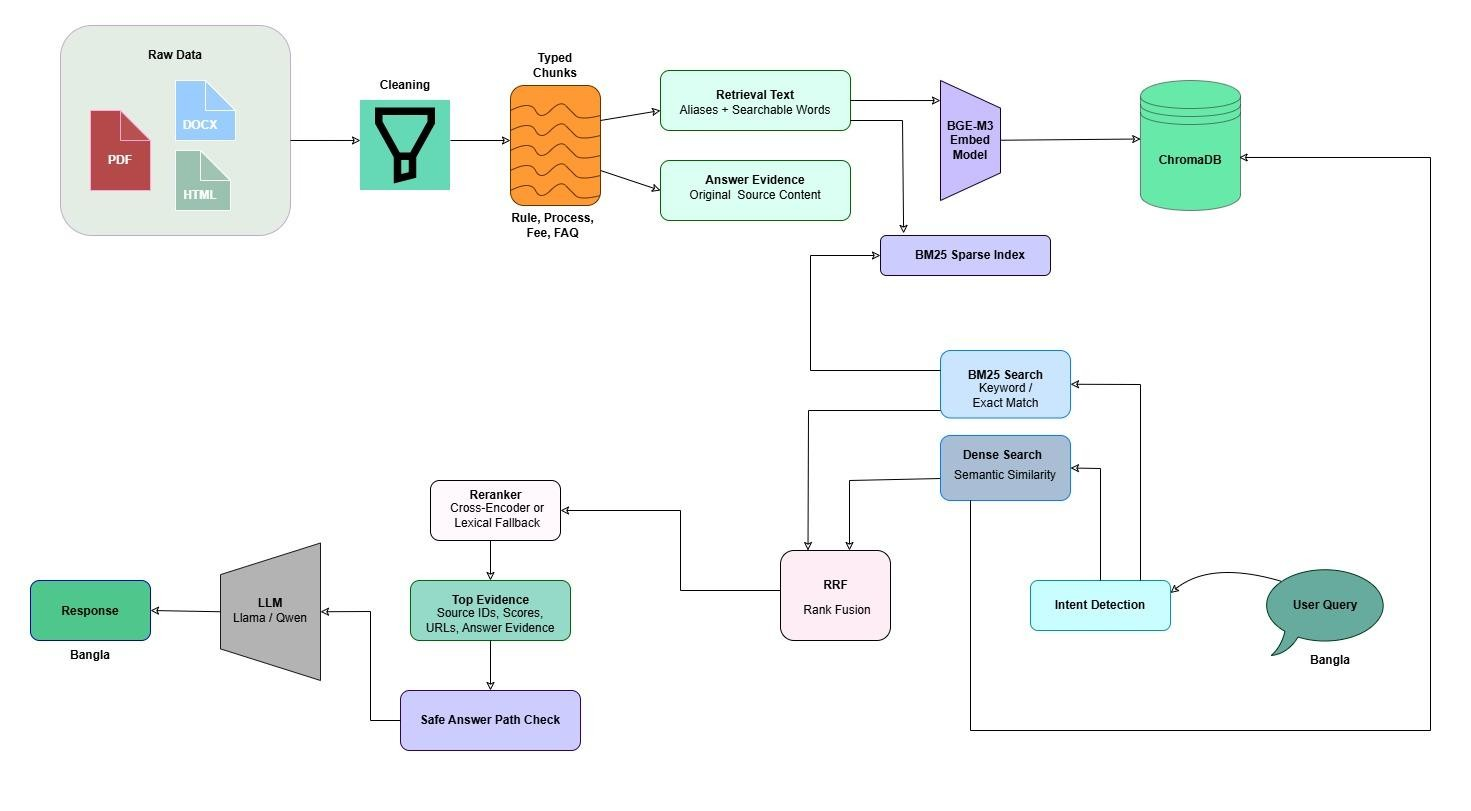
\includegraphics[width=\textwidth]{updated_p2_architecture_diagram.png}
    \caption{Proposed CivicRAG architecture for the birth registration domain. The offline indexing pipeline is separated from the online question-answering pipeline so that retrieval quality and generation quality can be evaluated independently.}
    \label{fig:civicrag_architecture_updated}
\end{figure}

Figure \ref{fig:civicrag_architecture_updated} shows the overall architecture of our current system. It is divided into two pipelines. The offline pipeline at first, processes raw government documents, cleans and chunks the data. Then, it creates two text versions per chunk, embeds the searchable text and stores it in a vector database. The online pipeline accepts a user query, detects language and civic intent, retrieves candidate chunks using dense and sparse retrieval. After that, it fuses ranked results, reranks evidence and finally generates a grounded response using either controlled answer paths or a local LLM.

\section{Preliminary Design Specification}

We considered and simulated several design solutions. The purpose of this comparison was not just to choose one final system but, additionally to justify why the selected design is appropriate for a factual Bangla government-service assistant.

\subsection{Design Solutions}

\begin{table}[h]
\centering
\caption{Design solutions considered for Civic.ai.}
\begin{tabular}{|p{3.2cm}|p{5.4cm}|p{5.2cm}|}
\hline
\textbf{Design Alternative} & \textbf{Description} & \textbf{Reason for Evaluation} \\
\hline
Dense-only RAG & Uses multilingual dense embeddings and vector similarity search. & Strong candidate for paraphrased Bangla queries where exact words may differ from source documents. \\
\hline
BM25-only RAG & Uses sparse lexical retrieval based on term matching. & Useful for exact government terms, legal rule numbers, fee terms and service names \cite{robertson2009bm25}. \\
\hline
Hybrid RAG & Combines dense retrieval and BM25 using rank fusion. & Provides a more robust architecture for future multi-domain expansion where both semantic and exact matching may matter. \\
\hline
CivicRAG & Adds metadata, source URLs, language and intent detection, reranking, safe answer paths and local LLM generation. & Selected design because it supports explainability, factual grounding and controlled answers for high-risk civic service questions. \\
\hline
\end{tabular}
\end{table}

The dense retrieval component is motivated by prior work on dense passage retrieval for open domain question answering \cite{karpukhin2020dpr} and sentence-level semantic representation learning \cite{reimers2019sbert}. In our current implementation, we used the BAAI/bge-m3 embedding model as it is designed for multilingual, multi-functionality and multi-granularity retrieval \cite{chen2024bgem3}. This is important for our Civic.ai system because our knowledge base is Bangla-heavy while user queries may appear in Bangla, English or code-mixed form.

The sparse retrieval component uses BM25, a strong probabilistic lexical retrieval baseline \cite{robertson2009bm25}. BM25 is specifically useful when a query contains exact service words, fee-related words, rule references, or official terminology. The simplified BM25 scoring function can be represented as:

\begin{equation}
BM25(q,d)=\sum_{t \in q} IDF(t)\cdot
\frac{f(t,d)(k_1+1)}
{f(t,d)+k_1(1-b+b\cdot\frac{|d|}{avgdl})}
\end{equation}

Here, $q$ is the query, $d$ is a document chunk, $f(t,d)$ is the frequency of term $t$ in chunk $d$, $|d|$ is the chunk length and $avgdl$ is the average chunk length. The parameter $k_1$ controls term-frequency and $b$ controls saturation and length normalization \cite{robertson2009bm25}.

To combine dense and sparse retrieval results, the system uses Reciprocal Rank Fusion (RRF). RRF combines multiple ranked lists without requiring the raw scores of different retrievers to be directly comparable \cite{cormack2009rrf}. In the current system, a weighted form of RRF is used:

\begin{equation}
RRF(d)=\sum_{r \in R}\frac{w_r}{k+rank_r(d)}
\end{equation}

where $d$ is a candidate chunk, $R$ is the set of retrievers, $w_r$ is the retriever weight, $k$ is the RRF constant, and $rank_r(d)$ is the rank of the chunk $d$ under retriever $r$. The original RRF formulation is unweighted, but the weighted version is useful for Phase 2 sensitivity analysis because it allows the dense and BM25 contributions to be tuned.

After going through fusion, a reranking stage is used to improve the order of candidate chunks. Cross encoder reranking is a common approach for passage reranking because it jointly scores the query and candidate passage \cite{nogueira2019passagebert}. The current Civic.ai implementation supports cross-encoder reranking when the local model is available and uses deterministic lexical/domain-aware fallback reranking for local reproducibility.

\section{Data Collection}

The current dataset focuses on Bangladeshi birth registration services. The sources include government service web pages, frequently asked questions, legal rules, fee information, application process documents, correction guidance and scanned or converted documents related to birth registration.

Four major raw data types were considered:

\begin{itemize}
    \item Bijoy-encoded PDF files.
    \item Converted DOCX files.
    \item Unicode HTML pages from government web portals.
    \item Scanned PDF or OCR-affected documents.
\end{itemize}

The current Phase 2 implementation primarily indexes manually reviewed and cleaned Markdown/JSON data. Raw scanned and converted files are retained for auditability, but only cleaned and structured content is used for the active vector database. This decision was made to reduce garbage-in-garbage-out errors in retrieval.

\subsection{Data Cleaning}

Civic service documents are often noisy and mixed or diverse. HTML files often contain menus, accessibility controls, footers, lists of unrelated services and navigation text. PDF and DOCX files sometimes contain broken formatting, repeated headings, encoding issues and OCR noise. Sometimes they include diagrams as well. Data cleaning is considered and treated as one of the core design steps rather than something minor since the quality of RAG heavily depends on the quality of retrieved data.

The data cleaning process includes:

\begin{itemize}
    \item Removing menus, footer blocks, accessibility controls and unrelated service lists.
    \item Removing gibberish texts and symbols and irrelevant text.
    \item Removing and converting all the non-Unicode/Bijoy texts where possible.
    \item Turning FAQ entries into individual question-answer units for creating safe answering paths.
    \item Preserving legal and procedural wording where exact phrasing is important.
    \item Eliminating OCR fragments, empty headings and duplicate content.
    \item Preserving official source URLs as metadata for explainability.
\end{itemize}

The goal of cleaning data is to prevent irrelevant and unnecessary texts from being embedded and retrieved. If noisy navigation or meaningless text is stored in the vector database the retriever may return chunks that match common words but do not answer the citizen's question or include gibberish texts in the response.

\begin{figure}[h]
    \centering
    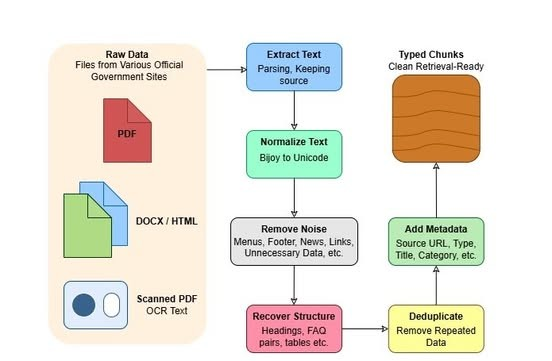
\includegraphics[width=0.88\textwidth]{updated_p2_data_cleaning_diagram.png}
    \caption{Data cleaning and preprocessing pipeline for proposed CivicRAG.}
    \label{fig:data_cleaning_pipeline_updated}
\end{figure}

\subsection{Data Transformation}

The data is transformed into retrieval friendly useful chunks after the cleaning process. Since there are various kinds of document types and one single chunking method is not suitable for that, we are using document-type-aware chunking.

\begin{table}[h]
\centering
\caption{Chunking strategy by document type.}
\begin{tabular}{|p{3.5cm}|p{5.1cm}|p{5cm}|}
\hline
\textbf{Document Type} & \textbf{Chunking Strategy} & \textbf{Reason} \\
\hline
FAQ JSON & Question-answer pair wise JSON chunk. & FAQ answers the most accurate answers and it is better to keep them intact. \\
\hline
Heading based Markdown & Section and subsection based chunking. & Preserves procedural structure and improves evidence interpretability. \\
\hline
Fee tables & Row wise chunks with fee metadata. & Fee questions require precise row level retrieval. \\
\hline
Legal/rule documents & Rule or paragraph group based chunks. & Legal evidence should be separated from unrelated sections. \\
\hline
Correction/application process documents & Step or condition based chunks. & Queries often include specific scenarios or require procedural steps. \\
\hline
\end{tabular}
\end{table}

Each chunk contains two separate text fields:

\begin{itemize}
    \item \textbf{retrieval\_text:} used for searching. It may include aliases, normalized terms and key words.
    \item \textbf{answer\_evidence:} used for generation. It contains original source content and is passed to the LLM for grounding.
\end{itemize}

This separation is required because aliases can elevate retrieval quality but the generator should not be grounded on artificial aliases. Therefore, the LLM receives original source content rather than expanded retrieval text.

\subsection{Data Integration}

All domain specific resources are organized under one domain. The current domain is:

\begin{center}
\texttt{domains/birth\_death\_registration/}
\end{center}

This folder holds cleaned Markdown/JSON files, generated chunks, ChromaDB vector storage, configuration files and evaluation datasets including raw documents. This design will help future multi domain expansion without having to create separate repositories. Future domains such as passport or BRTA as discussed can be added as new domain folders with their own data and configuration files.

\subsection{Data Reduction}

In this project, data reduction does not actually mean numerical dimensionality reduction. Instead, it means reducing irrelevant document noise and gibberish texts before indexing and reducing retrieved candidate chunks before generation. The important reduction decisions are:

\begin{itemize}
    \item Eliminating duplicate and irrelevant government website boilerplate.
    \item Removing duplicate FAQ content where the same question/answer appears in multiple sources.
    \item Splitting long documents into focused evidence units.
    \item Using fine tuned top-k retrieval to avoid sending too much context to the generator.
    \item Applying reranking and intent based boosting to prioritize the most relevant evidence instead of blindly sending the retrieved evidence.
\end{itemize}

Data Reduction is necessary because long or noisy retrieved data can confuse LLM generation. In a government service system, the answer should be precise and provide enough information but controlled because the actually answer should not be influenced or overshadowed by the unrelated chunks.

\subsection{Summary of Preprocessed Data}

The final preprocessed data contains Bangla heavy birth registration chunks. The major chunk categories are FAQ, legal rules, fee rows, correction steps, application steps, portal guidance and general service information. Each chunk holds metadata such as source ID, document type, section title, category and source URL.

For Phase 2 evaluation, a 58-question Bangla paraphrase evaluation set was created from 19 grouped birth certificate related problems. These questions are designed to evaluate whether the system can retrieve the same expected evidence when a citizen asks the same problem in different wording and even if it does how well it can do it.

\section{Implementation of Selected Design}

The selected design is CivicRAG, a modular local RAG system for government service question answering. The implementation consists of six main modules:

\begin{enumerate}
    \item \textbf{Data processing module:} reads cleaned Markdown and JSON files and converts them into typed chunks.
    \item \textbf{Embedding module:} embeds \texttt{retrieval\_text} using BAAI/bge-m3 \cite{chen2024bgem3}.
    \item \textbf{Indexing module:} stores dense vectors in ChromaDB and builds a BM25 sparse index.
    \item \textbf{Retrieval module:} retrieves candidates using dense search, BM25 search, or hybrid RRF search.
    \item \textbf{Reranking and safety module:} reranks candidates and checks whether a controlled answer path is available.
    \item \textbf{Generation module:} produces a final answer using local LLMs when a controlled answer is not available.
\end{enumerate}

The current local LLM backends are llama3.2, llama3, and qwen2.5:7b. Llama-based models are used as local open-weight baselines \cite{dubey2024llama3}, while Qwen2.5 is included as an alternative multilingual local model \cite{qwen2025qwen25}. The default generation temperature is set to 0.05 since government service queries require precise and consistent answers rather than creative answers. This low temperature eliminates the randomness.

For high-confidence civic intents such as fee questions, lost certificate questions, correction questions and application-process based questions the system can use safe answer paths. These paths reduce unnecessary LLM intervention by producing answers directly from selected evidence patterns. Retrieved evidence is sent to the local LLM with a strict grounding prompt to generate an answer if no safe path is found.

Generation quality is decided to be evaluated using metrics such as answer correctness, answer relevance, faithfulness and qualitative human review. RAG-specific evaluation frameworks such as RAGAS emphasize faithfulness, answer relevancy and context quality for retrieval augmented systems \cite{es2024ragas}.

Therefore, the Phase 2 implementation satisfies the design requirement of evaluating multiple alternative solutions before selecting the final architecture. Dense-only retrieval currently has the highest score on all fields, therefore, is the strongest retrieval baseline on the single domain Bangla evaluation set. Although CivicRAG remains the chosen system design since it is more explainable, supports source grounded responses and is better prepared for future multi-domain civic service expansion.

\section{Preliminary Evaluation}

A curated Bangla evaluation set was created to simulate real citizen questions. The current evaluation set contains 58 paraphrased questions. These questions cover application processes, correction cases, lost certificate cases, fees, legal conditions, online visibility problems and document requirements.

The retrieval alternatives were evaluated using ranking metrics commonly used in information retrieval, including Hit@k/Recall@k, Mean Reciprocal Rank (MRR), normalized Discounted Cumulative Gain (nDCG) and Context Precision \cite{manning2008ir,voorhees1999trec8qa,jarvelin2002ndcg}. The main retrieval results are shown in Table \ref{tab:retrieval_comparison_updated}.

\begin{table}[h]
\centering
\caption{Retrieval variant comparison on the 58-question Bangla evaluation set.}
\label{tab:retrieval_comparison_updated}
\begin{tabular}{|l|c|c|c|c|}
\hline
\textbf{Method} & \textbf{Hit@1} & \textbf{Hit@5} & \textbf{MRR} & \textbf{nDCG@5} \\
\hline
BM25-only & 0.5345 & 0.7586 & 0.6132 & 0.6112 \\
\hline
Dense-only & 0.7931 & 0.9828 & 0.8707 & 0.8693 \\
\hline
Hybrid RRF & 0.7414 & 0.9483 & 0.8193 & 0.8139 \\
\hline
\end{tabular}
\end{table}

The result shows that dense-only retrieval currently performs best for the birth registration evaluation set. This is reasonable because many evaluation questions are slightly modified or paraphrased Bangla questions, where semantic similarity is more important than exact word overlap. However, hybrid retrieval remains part of the selected design because future multi-domain expansion may increase lexical ambiguity. For example, different government services may contain semantically similar instructions but domain-specific terms such as passport, driving license, birth registration, death registration, fee, correction, or application. In such settings, sparse retrieval can help preserve exact domain signals.

The following metrics were used:

\begin{equation}
Recall@k = \frac{\text{Number of queries where a relevant chunk appears in top }k}{\text{Total number of queries}}
\end{equation}

\begin{equation}
MRR = \frac{1}{|Q|}\sum_{i=1}^{|Q|}\frac{1}{rank_i}
\end{equation}

MRR measures how early the first relevant chunk appears in the ranked list \cite{voorhees1999trec8qa,manning2008ir}. For ranking quality with graded relevance, nDCG is used:

\begin{equation}
DCG@k = \sum_{i=1}^{k}\frac{2^{rel_i}-1}{\log_2(i+1)}
\end{equation}

\begin{equation}
nDCG@k = \frac{DCG@k}{IDCG@k}
\end{equation}

where $rel_i$ is the relevance score of the result at rank $i$, and $IDCG@k$ is the ideal DCG at rank $k$ \cite{jarvelin2002ndcg}.

The generation side design was also examined through context size testing. The goal was to determine how many retrieved chunks should be sent to the answer generator. Table \ref{tab:topk_context_updated} shows the trade-off between evidence coverage and context precision.

\begin{table}[h]
\centering
\caption{Generation context top-k coverage.}
\label{tab:topk_context_updated}
\begin{tabular}{|c|c|c|}
\hline
\textbf{k} & \textbf{Expected Source in Context} & \textbf{Context Precision@k} \\
\hline
1 & 0.7414 & 0.7414 \\
\hline
3 & 0.8793 & 0.3621 \\
\hline
5 & 0.9483 & 0.2448 \\
\hline
8 & 0.9828 & 0.1616 \\
\hline
\end{tabular}
\end{table}

The results show that larger context sizes improve the chance of including the expected evidence but also introduce more irrelevant chunks. The current selected value is $k=3$ for generation because it is conservative and reduces noise. However, $k=5$ is a candidate for future testing because it improves expected-source coverage.


\printbibliography

\end{document}
